\documentclass[italian]{beamer}
%\documentclass[italian,handout]{beamer}

\usepackage[utf8]{inputenc}

% Uso un file unico, non serve molto

\title[Bitcoin]{Analisi di Bitcoin}
\subtitle{Anonimato, Sicurezza e Sviluppi Futuri}
\author[Paoluzzi Matteo]{Paoluzzi Matteo}
\institute[UniUD]{Università degli Studi di Udine\and{}Relatore:\\{}Dott. Ivan Scagnetto}
\date[2014/04/03]{IV Sessione di Laurea AA 2012/2013, Aprile 2014}
\subject{Bitcoin}

\usepackage{color}
\usepackage{default}
\usepackage{pres_commands}
\usepackage{ragged2e}
\usepackage{subcaption}
%\usepackage{pres_uniudtesi}
\usetheme{Madrid}

\definecolor{arancione}{HTML}{FF7F00}
\definecolor{giallo}{HTML}{FFFF33}
\definecolor{rosso}{HTML}{E4191B}
\definecolor{verde}{HTML}{4CAE4A}
\definecolor{viola}{HTML}{984DA3}

\graphicspath{{./img/}}

\hypersetup{
  pdfstartview={Fit},
  pdftitle={Presentazione della Tesi ``Analisi di Bitcoin: Anonimato, Sicurezza e Sviluppi Futuri``},
  pdfauthor={Paoluzzi Matteo},
  pdfsubject={Modello di presentazione di Tesi al computer},
  pdfkeywords={LaTeX pdf presentazione tesi laurea}}
  
\begin{document}

\frame{\titlepage}

\begin{frame}{Di cosa si tratta} % 1
\justifying
Una valuta elettronica basata su crittografia a chiave pubblica progettata per:
\begin{itemize}
\justifying
 \item Proteggere l'identità degli utenti sfruttando \textbf{indirizzi} anonimi.
 \item Essere indipendente da qualsiasi istituto di credito.
 \item Essere immune dal rischio di inflazione.
 \item Funzionare su base P2P in modo pubblico, sicuro e verificabile.
\end{itemize}
\end{frame}

\begin{frame}{Indirizzi} % 2
\justifying
L'anonimato dell'utente viene implementato tramite stringhe di testo note come indirizzi.
\begin{itemize}
\justifying
 \item Un indirizzo viene generato a partire da una coppia di chiavi pubbliche e private.
 \item Tutte le \textbf{transazioni} di BTC avvengono da e verso indirizzi, senza divulgare informazioni sull'identità delle parti coinvolte.
 \item Le chiavi di cifratura consentono di spendere il denaro ricevuto e impedire che il denaro inviato finisca ad un destinatario diverso da quello desiderato.
 \item Ogni utente è incoraggiato ad avere molteplici indirizzi, mantenendo sicure le porzioni private delle chiavi appositamente generate.
\end{itemize}
\end{frame}

\begin{frame}{Transazioni} % 3
\justifying
\begin{itemize}
\justifying
 \item Sono identificate da un hash calcolato su un sottoinsieme di dati in modo da fissare alcune proprietà specifiche.
 \item Gli output contengono le BTC inviate e lo script che il destinatario deve eseguire per spendere le BTC.
 \item Con gli input si firmano gli output di transazioni precedentemente ricevute dimostrando di esserne il proprietario.
 \item Se l'input è maggiore dell'output, il resto diventa una \textbf{transaction fee} donata a chi trova il \textbf{blocco} contenente la transazione.
\end{itemize}
\begin{figure}[htbp]
\centering
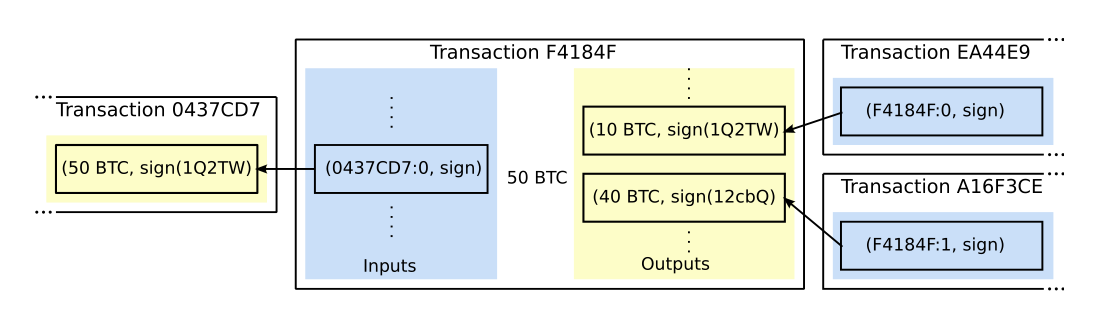
\includegraphics[width=\textwidth]{bitcoinpropagation_1.PNG}
\end{figure}
\end{frame}

\begin{frame}{Blocchi} % 4
\justifying
Le transazioni vengono raccolte in blocchi che risultano validi se il loro hash non supera un determinato target:
\begin{itemize}
\justifying
 \item Trovare tale hash è un'operazione detta \textbf{mining} configurato ridimensionando il target ogni 2016 blocchi in modo da generare in media un blocco ogni 10 minuti.
 \item Il nodo che trova il blocco viene premiato con una quantità fissa di BTC e con le transaction fee.
\end{itemize}
Nell'insieme i blocchi formano una \textbf{blockchain} il cui scopo è fissare le transazioni nel tempo rendendone computazionalmente quasi impossibile la modifica.
\begin{figure}[htp]
\centering
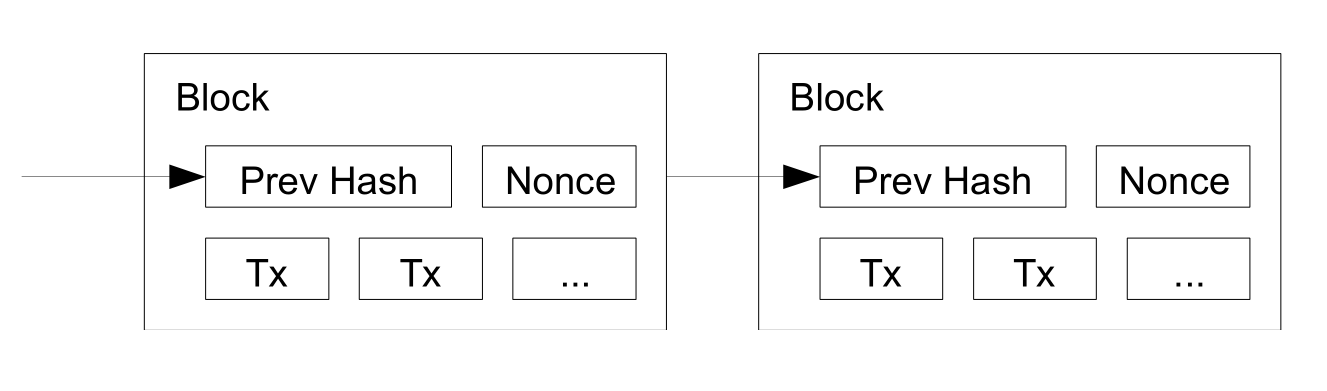
\includegraphics[scale=0.25]{bitcoin_p3_1.PNG}
\end{figure}

\end{frame}

\framedgraphic{Infografica}{transactions_ABC} % 5

\begin{frame}{Vulnerabilità} % 6
\justifying
 \begin{description}
 \justifying
  \item[Double-Spending] Inoltrare più transazioni con lo stesso input in modo che solo quella più conveniente per il mittente venga inclusa in un blocco senza che il destinatario se ne accorga. Senza contromisure e con adeguata preparazione, l'attacco ha una probabilità di successo del 90\%.
  \item[History Revision] Creare una blockchain alternativa che modifica l'intera storia delle transazioni da un dato blocco in poi. Una blockchain alternativa può verificarsi spontaneamente con una probabilità del 1.78\% ma si risolve automaticamente.
  \item[Portafogli] Contengono le chiavi private neccessarie per spendere le proprie BTC e sono quindi un obiettivo sensibile da tenere il più possibile sicuro e lontano da pericoli.
 \end{description}
\end{frame}

\begin{frame}{Protezione} % 7
\justifying
 \begin{description}
 \justifying
  \item[Double-Spending] Collegandosi ad un gran numero di nodi fidati, bloccando le comunicazioni in ingresso e attendendo numerose conferme di ogni transazione è possibile di fatto annullare le probabilità di successo di un attacco doppia-spesa.
  \item[History Revision] È possibile dimezzare la frequenza di blockchain alternative spontanee velocizzando la propagazione dei messaggi in rete. Le blockchain arbitrarie non possono essere bloccate, ma è estremamente improbabile (per ora) che un tale attacco possa avere luogo.
  \item[Portafogli] Oltre le classiche opzioni di cifratura, è possibile salvare il portafogli in computer mai collegati in rete (\textbf{cold storage wallet}) oppure usare indirizzi ''receive main - send once`` stampati unicamente su carta (\textbf{paper wallet}).
 \end{description}
\end{frame}

\begin{frame}{Privacy} % 8
\justifying
Il sistema di indirizzi adottato è simile a quello dei conti bancari in Svizzera: numeri di conto non collegabili direttamente a persone.\\
Ma il sistema di cifratura a chiave pubblica permette di stabilire se indirizzi diversi hanno il medesimo proprietario:
\begin{itemize}
\justifying
 \item Una transazione contenente più indirizzi in input indica che tali indirizzi appartengono tutti al creatore della transazione stessa.
 \item Se una transazione contiene un output molto piccolo e destinato ad un indirizzo mai visto prima, probabilmente tale indirizzo è stato creato appositamente dal creatore della transazione per raccogliere il resto.
\end{itemize}
Creando un grafo delle transazioni pubblicamente disponibile e applicando le aggregazioni descritte, è possibile creare un secondo grafo approssimato rappresentante il flusso di monete tra utenti invece che tra indirizzi. Unendo questi due grafi ad altre fonti esterne potrebbe essere possibile identificare effettivamente un utente e tracciarne le attività.
\end{frame}

\begin{frame}{Esempio reale: un furto} % 9
\begin{figure}[ht]
  \centering
  \begin{subfigure}{0.45\textwidth}
    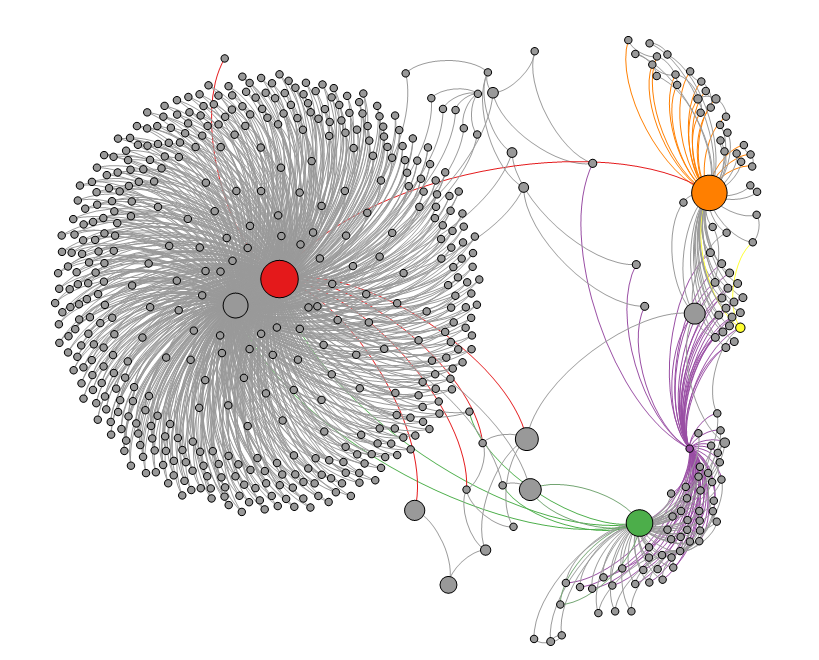
\includegraphics[width=\textwidth]{anonimato_1_11.PNG}
    \caption*{
    \textcolor{verde}{Vittima}\\
    \textcolor{rosso}{Presunto ladro}\\
    \textcolor{viola}{Slush Pool}\\
    \textcolor{arancione}{LulzSec}\\
    \textcolor{giallo}{Sconosciuto}
    }
  \end{subfigure}
  \begin{subfigure}{0.45\textwidth}
    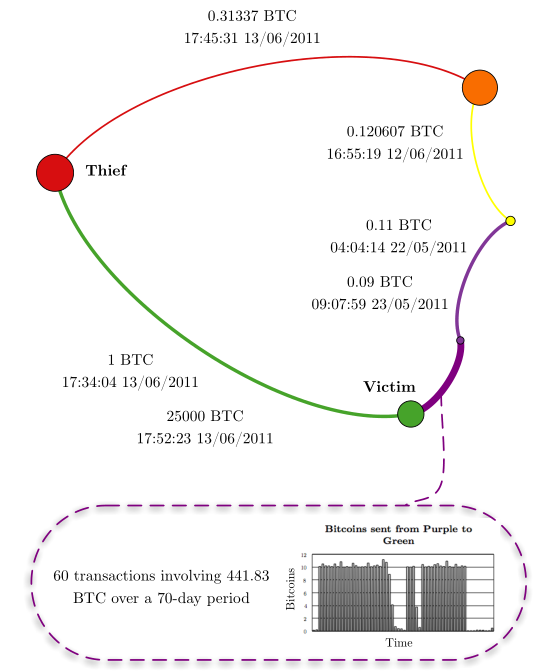
\includegraphics[width=\textwidth]{anonimato_1_12.PNG}
  \end{subfigure}
\end{figure}
\end{frame}

\framedgraphic{Furto: transazioni seguenti}{anonimato_1_13} % 10


%%%%%%%%%%%%%%%%%%%%%%%%%%%%%%%%%%%%%%%%%%%%%%%%%%%%%%%%%%%%%%%%%%%%%%%%%%%%%%%%%%%%
% \item Formula che appare un poco per volta:
% \pause
% \parstepwise{
% $$
%   1\step{{}+2}
%   \step{{}+3} \step{{}+4}\step{{}+\cdots+n}
%   \step{{}={}}
%   \step{\sfondogiallo{$\displaystyle\frac{n(n+1)}{2}$}}
% $$
% }
%
%\pageTransitionGlitter{0}
% il comando \newframe e' come \newpage,
% ma non avanza il numero di pagina.
% Puo' servire per fare cambiamenti incrementali
% a una pagina, quando \pause o \stepwise non
% bastano. In questo esempio \pause non va bene
% perche' qui bisogna aggiungere un paragrafo
% ma allo stesso tempo  cambiare la figura che
% sta in cima alla pagina. Macchinoso da scrivere,
% ma puo' valerne la pena.
%
%\newframe
%
%\sfondogiallo{\rosso{\textit{coincidono:}}}
%
% Le transizioni si attivano al /pause
%\pageTransitionWipe{0}
%\pageTransitionWipe{180}
%\pageTransitionSplitVO
%\item {\setlength{\baselineskip}{2\baselineskip}
%Vedere la documentazione del pacchetto \textcolor{darkorange}{\texttt{texpower}}.
%}
%\pageTransitionReplace
%\pageTransitionBoxI
%%%%%%%%%%%%%%%%%%%%%%%%%%%%%%%%%%%%%%%%%%%%%%%%%%%%%%%%%%%%%%%%%%%%%%%%%%%%%%%%%%%%
\end{document}
